 \documentclass{article} % For LaTeX2e
\usepackage{cos424,times}
\usepackage{url}
\usepackage{graphicx}
\usepackage{hyperref}
\usepackage{amsmath}

\usepackage{biblatex}
\bibliography{bib.bib}

\title{Already Asked: Detecting Duplicate Question Pairs in the Quora Dataset}


\author{
Meir Hirsch \\
Computer Science\\
\texttt{ehirsch@} \\
\And
Charles Stahl \\
Physics \\
\texttt{cnstahl@} \\
\And
Kenan Farmer\\
Computer Science \\
\texttt{kfarmer@}\\
}

\newcommand{\fix}{\marginpar{FIX}}
\newcommand{\new}{\marginpar{NEW}}
\newcommand{\wordtvec}{\texttt{word2vec}}

\begin{document}

\maketitle

\begin{abstract}
This project uses a dataset posted on Kaggle~\cite{kaggleComp} to detect duplicate question pairs on Quora, a popular question-and-answer website~\cite{quora} that received 100 million monthly unique visitors as of March 2016~\cite{qvisit}. The training data includes 404,290 question pairs chosen from 537,933 questions, classified as duplicates or not. The testing set was 2.3 million unlabeled pairs, with 4.2 million unique questions. The methods we used consisted of counting the overlapping words, bag-of-words (BOW) methods, \wordtvec, and word nets to reduce the dimensionality of the data. We then used multinomial na\"ive Bayes, logistic regression with and without stochastic gradient descent, and random forest models to classify duplicates. The best method was BOW with logistic regression.
\end{abstract}

\section{Introduction}

Quora is a website that strives to connect people from different backgrounds to be able to answer questions whose answers are ``either locked in people’s heads, or only accessible to select groups" \cite{quora}. Questions range from ``What is the most embarrassing text message you have sent to the wrong person?" to ``How do I identify entities in natural language search query?" to ``Do virtual particles and energy in vacuum really exist?"

Once a question is answered, any other person should be able to find the response, and the question never needs to be asked again. However, sometimes people are unable to find the questions they want and end up asking the same question again. This counteracts Quora's vision of having ``only one version of each question\dots [not] a left wing version, a right wing version, a western version, and an eastern version"~\cite{quora}. Duplicate questions also waste resources for the website, the answerers, and future viewers who will either see one answer or the other, but not the canonical response the website has to offer.

Quora currently identifies duplicate questions with a Random Forest model~\cite{kaggleComp}. Quora does not have a method for users to mark questions as duplicates, although they allow users to redirect questions. Stack Exchange, a similar question-answer website, does allow users to mark questions as duplicates~\cite{stackdup}. 

To improve their duplicate identification, Quora released a dataset of question pairs on Kaggle, a platform for data science-based prediction and classification problems~\cite{kaggleComp}. In this project, we identify features and statistical machine learning methods that effectively detect duplicates in the Quora questions. This paper first explores related duplicate detection projects and explains the data used. It then describes the features we chose to extract from the data, with a special emphasis on \wordtvec, a method for word embedding. We then present results, along with analysis and conclusions drawn. 

\section{Related Work}

Zhang, et. al. created a duplicate detection tool for use on the Stack Overflow (SO), a website in the Stack Exchange network~\cite{Zhang2015}. It uses the title, content, and tags of the questions to assign topics using Latent Dirichlet Allocation (LDA)~\cite{Blei03}. The method then predicts duplicates by comparing topic distributions.

Since Quora questions include only the single sentence question, they are nearly equivalent to just the title of an SO question. The tags and content on SO are more significant and better indicate the meaning of a question, meaning this method is not useful on the Quora dataset. This analysis also only used bag-of-words text similarity and LDA to detect duplicates.

An earlier paper focused on detecting duplicate bug reports~\cite{Runeson2007}. The motivation of this problem is similar, centering on the wasted time used to identify and respond to duplicate reports. This study used standard NLP tools along with a term-frequency vector space to define distance measured between reports. Another paper contains a review of relevant similarity measures from 2008 can be found in~\cite{acha08}. Quora also released a document explaining some basic deep learning methods to use~\cite{quora_eng}.

\section{The Data}

Each line of the training set consists of a pair ID, two question IDs, the text of two questions, and an indication of whether the questions have the same intent. The testing set only contains a pair ID and the text of two questions. The questions are usually between 7 and 12 words in length. As mentioned in the abstract, the testing set is significantly larger than the training set. The goal of the competition is to submit a file with pair IDs from the testing set along with a probability that that pair is a duplicate. It then reports the log loss calculated on 35\% of the set, reserving the other 65\% for the final ranking.

We decided to approach the problem differently than the method in~\cite{Zhang2015}. While they chose to model each question and then look for duplicates, we decided that method would not be as helpful. Since we are looking for duplicates rather than related questions, the all-to-all interactions would be very sparse. Therefore we chose to model the problem as binary classification on question pairs, extracting features from each pair. 

As in all machine learning projects, we need a metric to assess the quality of our model. We decided to use the competition's metric, the log loss of the probabilities of duplicates. This is defined as the negative sum of the probabilities we assign to the correct class, or
\begin{align}
\text{log loss} = -\frac{1}{N}\sum_n \left(y_n\log p_n + (1-y_n)\log(1-p_n)\right),
\end{align} 
where $y_n$ is the true class label and $p_n$ is the probability we assign to the pair of being a duplicate. 

We did however impose some restrictions on what information we would use. The competition exposed the text of the testing data but not the labels. Since the text of the testing data would be available in a real-world application of this problem, we decided that training models on this text would not be considered double-dipping, especially since we did not have labels for this text. 

It is possible, however, to extract the proportion of positive samples in the testing data through the reported log loss. If a submission consists of only a constant probability $p$, the log loss is
\begin{align}
\text{log loss} &= -\frac{1}{N}\sum_n \left(y_n\log p + (1-y_n)\log(1-p)\right)
	\nonumber\\
&= -\left(y'\log p + (1-y')\log(1-p)\right),
\end{align}
or 
\begin{align}
y' = \frac{\text{log loss} + \log(1-p)}{\log(1-p)-\log p},
\end{align}
where $y'$ is the proportion of positive test samples. A constant test prediction of 0.75 results in a log loss of 1.19485, meaning the proportion of positive test samples is 0.17426. Simply guessing this probability results in a log loss of 0.46258. 

We could in principle use this data to structure our submissions, so that they have a mean of 0.17426. However, since this data would not be accessible in the real world, we decided to not use it in our methods. Furthermore, the proportion in the set used for final ranking may be different that in the 35\% used for initial ranking.

We also chose not use use neural networks for prediction, despite the fact that most people at the top of the leaderboard probably did. This allowed us to have more easily interpretable results, but led to less-than-stellar submissions. 

\section{Methods}

The training data was read from csv files using Pandas~\cite{pandas}. Lemmatization and stop word removal was completed using the Spacy package, a package for ``Industrial-Strength Natural Language Processing"~\cite{spacy}. Another NLP tool used is the Natural Language Toolkit~\cite{nltk}.

\subsection{Feature Engineering} \label{sub:features}

Our na\"ive method was to count the number of words in common between the two questions in the pair. A slight variant on this was listed on Kaggle as a benchmark. We improved upon this by counting how many words are in common and how many are distinct, and then by separately counting the number of nouns, verbs, named entities and \_\_\_\_ in common between questions. We also included a count of how many of each part of speech occurs in one sentence but not the other. 

Our next was a BOW method, but instead of defining an individual bag for each question, we defined a bag for each pair of questions, only including words unique to one question or the other. We then defined a second bag, only including distinct words. The second bag did not treat words unique to sentence $a$ differently from those unique to sentence $b$.

A promising source of features was word embeddings, using Gensim's implementation of \wordtvec~\cite{gensim} and Spacy's built-in \wordtvec\ embedding. Word embeddings were introduced in the early 2000's to address the high rate of orthogonality inherent in BOW-based methods~\cite{Bengio03}. Since the BOW methods only look at counts of words, the meanings of the words are not encoded. This leads to high-dimensional, very sparse vectors, leading to the high rate of orthogonality.

A canonical example is from~\cite{kusner15}. Consider the two sentences
\begin{center}
\text{Obama speaks to the media in Illinois.}
\end{center}
and 
\begin{center}
\text{The President greets the press in Chicago}.
\end{center}
These sentences are orthogonal in a space that assigns each word its own dimension. Therefore they have a cosine similarity of 0. However, an effective similarity measure should indicate that these sentences are very closely related.

Word embedding looks at a large corpus to find how different words are related and connected. It creates a space with dimension lower than the number of words, so that each word is represented as a non-sparse vector. Words with similar meaning are closer in this space, giving a high similarity score for the above sentences. Furthermore, algebraic manipulation of these vectors carries significance. Ideally this would lead to usable analogies, such as \textit{Paris - France + Italy = Rome}, or \textit{suhi - Japan + Germany = bratwurst}.

The 2013 implementation from Google, called \wordtvec, uses a shallow neural network to embed words in the vector space~\cite{word2vec}. For a detailed description of \wordtvec\ see subsection~\ref{sub:detail}.

From the \wordtvec\ embeddings of the words in each question, we can compute the word mover's distance (WMD)~\cite{kusner15}. For sentences $M$ and $N$ of length $J$ and $K$ with words $m^j$ and $n^k$, the WMD is defined as 
\begin{align}
\text{WMD}(M,N) = \sum_{j=1}^J\min_{n^k\in N}\left|m^j-n^k\right|,
\end{align}
the total distance needed to move each word in $M$ to the nearest word in $N$.

The WordNet methods were implemented using NLTK. WordNet is a database of English words and meanings created manually at Princeton~\cite{wordnet}. Words are arranged in syntactic sets based on parts of speech, and connected to their synonyms and antonyms. NLTK then uses the database to find similarity measures between words using these groups of words. 

\subsection{One method in detail: \wordtvec} \label{sub:detail}

The \wordtvec\ method introduced in subsection~\ref{sub:features} merits further discussion. Training the model uses a 2-layer neural network. The implementation we used was hidden, but understanding the working is still useful. The presentation here is based on tutorials from~\cite{tensorflow} and~\cite{mccormick}.

As previously mentioned, the motivation of word embeddings is to find a vector representation for words that is not as sparse as count-based methods. To do this, we first train a neural network to learn the relationships between words and environments, or histories. The Continuous Bag-of-Words model predicts words based on environments while the skip-gram model predicts environments based on individual words. This uses a 2-layer neural network, as seen in figure~\ref{fig:skipgram}. 

\begin{figure}[h]
	\centering
	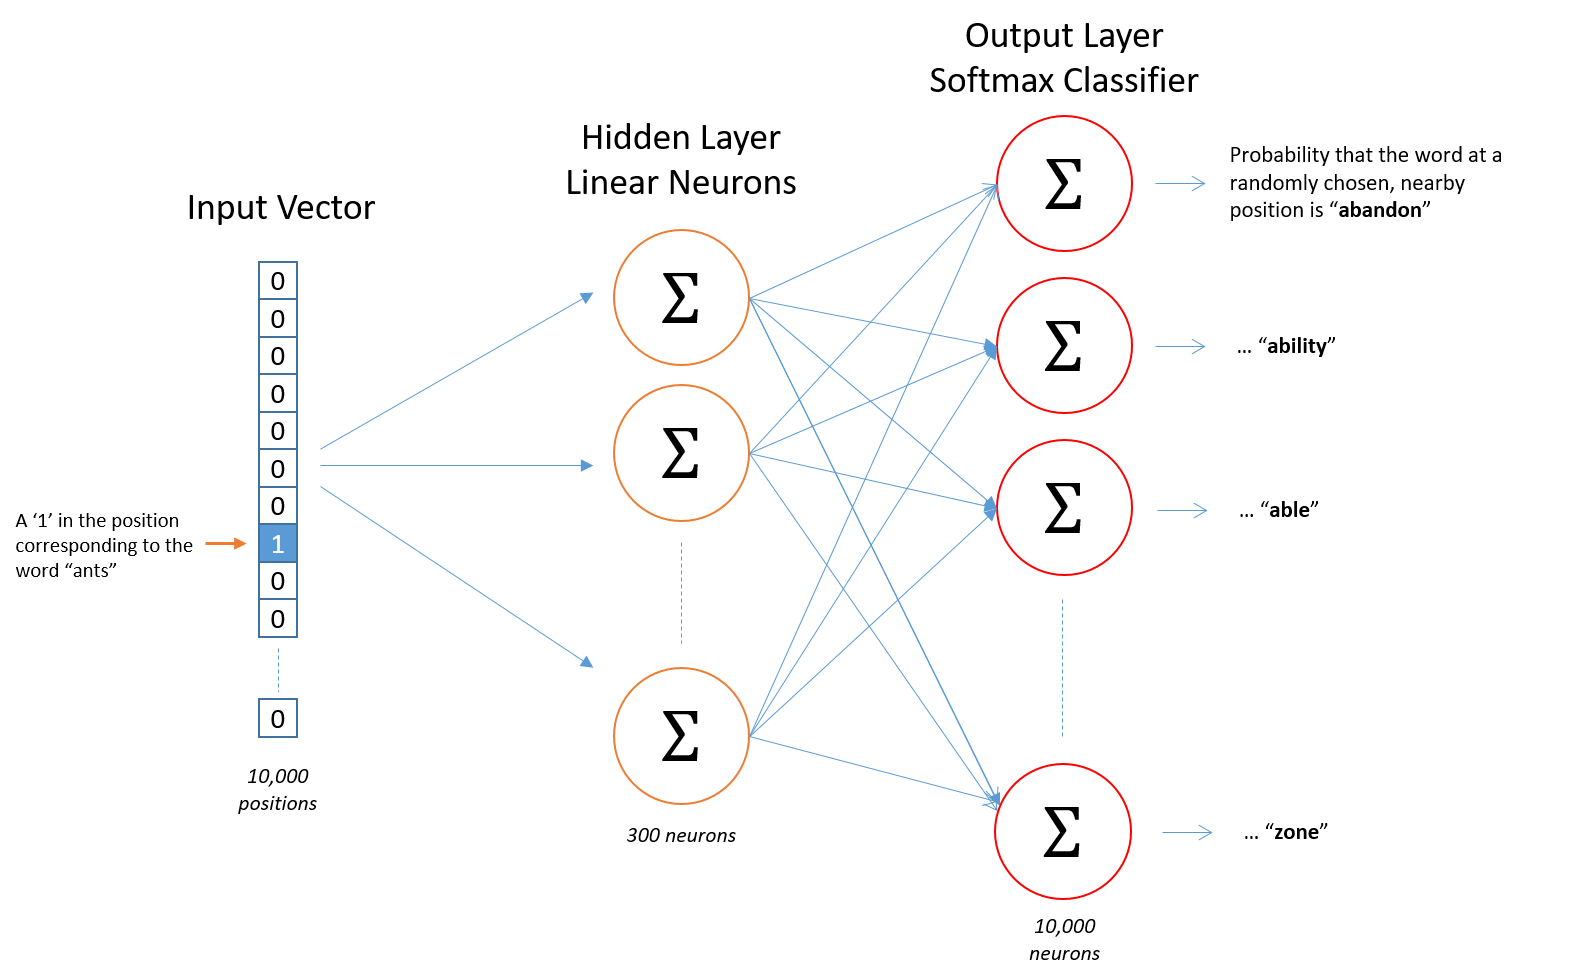
\includegraphics[width=.5\textwidth]{skip_gram_net_arch}
	\caption{\textbf{Architecture for Skip-Gram Model.} The network contains two layers after the input vector. The output layer predicts the word, but the hidden layer contains the weights used for embedding. Image from~\cite{mccormick}.}
	\label{fig:skipgram}
\end{figure}

For a vocabulary of size $N$, the input is a $N$-component vector one-hot encoded for the input word $v$. The output vector also has $N$ components, each of which is the probability that a word in the environment of $v$ is the word corresponding to that component. 

Neural networks work using neurons, each of which has an input and weights. In the skip-gram architecture, each neuron in the hidden layer has the input vector as its input. Each neuron in the output layer has all hidden neurons as input. Each training step consists of choosing a word to train on, feeding it though the network, and calculating the loss of the output vector. The parameters $\theta$ of the model are then moved slightly in the direction of the gradient of the loss w.r.t. $\theta$.

Once the model is trained, the word embeddings can be extracted. Consider a model with $H$ hidden neurons. Since each is linear, the vector of activations $h$ is just
\begin{align}
h=Mv, \label{eqn:hidden}
\end{align}
where $M$ is a $H$ by $N$ matrix containing the weights of all neurons. Since the words are one-hot encoded in $v$, the output of the hidden layer will be a single column of $M$. 

The output of the network is a softmax layer defined such that each component is between 0 and 1, and the components sum to 1. These are interpreted as the probability that a word will appear in the environment of the input word.

The key to \wordtvec\ is in looking at the output of the hidden layer. In fact, once the model is trained the output layer can be removed. Consider two words whose output vectors are similar. This means the two words are likely to occur in similar environments. This can be interpreted as the two words being semantically related. 

The last step, to actually obtain dense representations of the words in a vector space, is to realize that since the output vector is a linear transformation of the output of the hidden layer, two words with similar weights in the hidden layer will be semantically related. As described after equation~\ref{eqn:hidden}, these outputs are just the columns of $M$, which can be called the word vectors. 

An impressive display of the significance of \wordtvec\ is the capability to form analogies through algebraic manipulation of vectors. For example, starting with the vector for ``Paris," one can subtract the vector for ``France" and add the vector for ``Italy." The nearest vector in the space will then be ``Rome." A list of such analogies is in table~\ref{tab:anal}, including the imperfect analogies.

\begin{table} [tb]
\centerline{
\begin{tabular}{|c||c|c|c|}
	\hline
	Relationship            &  Example 1             &  Example 2             &   Example 3           \\
	\hline
	France - Paris          &   Italy: Rome & Japan: Tokyo  & Florida: Tallahassee    \\
	big - bigger            & small: larger & cold: colder  & quick: quicker \\
	Miami - Florida         & Baltimore: Maryland  & Dallas: Texas     & Kona: Hawaii    \\
	Einstein - scientist    & Messi: midfielder & Mozart: violinist & Picasso: painter \\
	Sarkozy - France        & Berlusconi: Italy & Merkel: Germany   & Koizumi: Japan  \\
	copper - Cu             & zinc: Zn          & gold: Au          & uranium: plutonium    \\
	Berlusconi - Silvio     & Sarkozy: Nicolas  & Putin: Medvedev   & Obama: Barack   \\
	Microsoft - Windows     & Google: Android   & IBM: Linux        & Apple: iPhone   \\
	Microsoft - Ballmer     & Google: Yahoo     & IBM: McNealy      & Apple: Jobs     \\
	Japan - sushi           & Germany: bratwurst & France: tapas    & USA: pizza      \\
	\hline
\end{tabular}}
\caption{\textbf{Analogy examples from \wordtvec}, taken from the initial \wordtvec\ paper,~\cite{word2vec}. Note the analogies are not perfect, but generally good.}
\label{tab:anal}
\end{table}

\section{Results}

The results for word count and BOW based methods are summarized in table~\ref{tab:res}.

\begin{table}[h]
\vspace{2mm}
\centerline{
\begin{tabular}{|c||c|c|c|c|c|c|c|}
	\hline
	Log loss     &  MNB   & LogReg &with SGD&RandForest& LDA & GBoost & Other \\
	\hline
	Word Count   & 0.6828 & 0.5440 & 0.5855 & 0.4089   &0.5584 &0.4663   & ---  \\
	Bag of Words & 0.4546 & 0.4277 & 0.5229 & 0.6083   &---  & --- & ---  \\
	BOW, tf-idf  & 0.45464 & 0.42771 & 0.52297 & 0.60837    & ---& ---& ---  \\
	\hline
	\hline
	Ensemble     & ---     & ---     & ---     & ---    & ---& ---    & 0.3826 \\
	\hline
	\end{tabular}}
	\caption{\textbf{Log loss results} for multinomial na\"ive Bayes, logistic regression with and without stochastic gradient descent, random forest, linear discriminant analysis, and gradient boost. The Ensemble method is described in subsection~\ref{sub:ense}.}
	\label{tab:res}
\end{table}

The ensemble method is an average of the best individual methods.

\subsection{Word Counts} \label{sub:count_res}

The word count method worked well as a baseline method. On the testing data, it did not perform as well as guessing the mean, but again this is because we did not adjust the mean of our predictions to match the empirical mean. Simple features of the number of shared words and the number of common words alone scored \_\_\_\_, while a method including all features scored a best of \_\_\_\_. 

The best classification method for the word count was a random forest. This is not surprising, because\_\_\_\_. ROC curves for both the word count and BOW methods can be seen in figure~\ref{fig:roc_wc}.

\begin{figure}[]
	\centering
	\includegraphics[width=.49\textwidth]{roc_bow}
	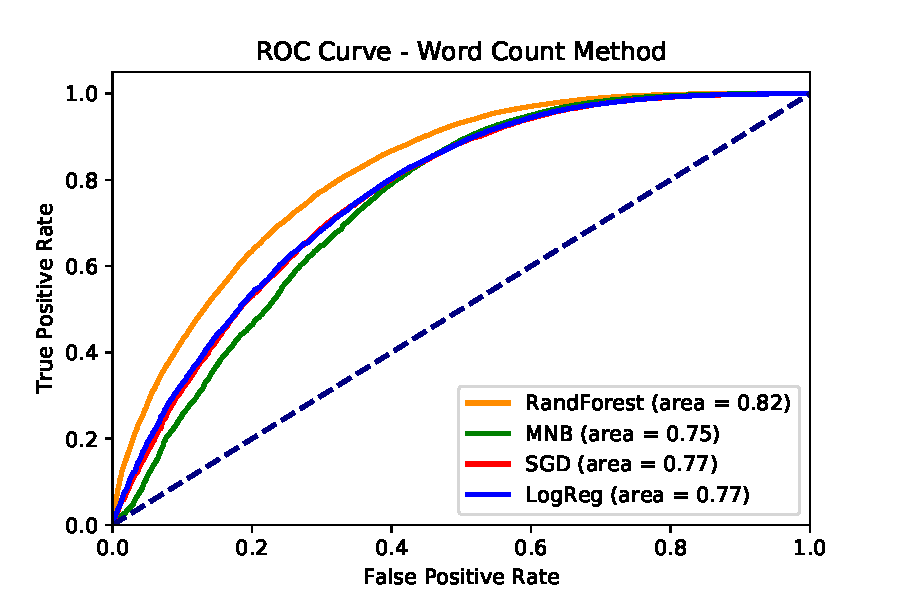
\includegraphics[width=.49\textwidth]{roc_wc}
	\caption{\textbf{ROC curves for word count and BOW methods.}}
	\label{fig:roc_wc}
\end{figure}

\subsection{Bag-of-Words} \label{sub:bow_res}

The Bag of word model is of width twice the vocabulary length, one half to represent the words that are in common between the two questions and one half to represent the words that differ between the two questions. This made the data quite large and immediately showed the problems associated with size in the Random Forest Regressor taking a large amount of time to run. In order to run the random forest classifier, we had to take out so much functionality that the method fell out of first place. The Multinomial Naive Bayes method ran the fastest out of the methods analyzed and gave surprising performance only to be bested by Logistic Regression for each feature model. The best performing model was logistic regression with a score of .41490 which is a surprising testament to counterintuitive performance of simple models.

Support Vector Machines were computationally too expensive to run any feature set.

\subsection{WordNet} \label{sub:wnet_res}
Our exploration of WordNet seemed promising from the beginning of the project and through feature planning. However, the vast scale of WordNet and various issues in contextualizing words made this intractable for our large dataset. The main problem is that each word can have different parts of speech or different \textit{meanings} leading to a vast number of synsets per word. In example, the word dog has 11 synsets to which it belongs in the english NLTK corpus. To calculate the WordNet measure of similarity we must filter through these to find the correct match of context. After investigating tools to accomplish this task, We found LESK a function in the NLTK package that resolves which synset to use given the word's context in the sentence. Quickly we found that LESK did not have enough context clues to resolve synsets.

After abandoning the sysnets we attempted to resolve with the most popular context and run with that. This also became too computationally expensive as each WordNet query required a search for the most specific common ancestor of the two words. This expensive query lead to run times of close to 5 hours for running on just the training data set. An expected 30 hours would be needed for running on the full training an testing dataset rendering this task unreasonable without access to servers.

%\footnote{We believe in reporting both our failures and our successes which unfortunately is a sparse characteristic in academia research today}
\subsection{\wordtvec}
The \wordtvec\ feature performance results were extremely puzzling. We expected \wordtvec\ to perform the best of all our engineered features as it has some interesting properties. With these properties, we engineered specific interpretable features of different structures to model the sentences after.

Once each word in a sentence is vectorized there are many ways to filter and evaluate the two collections of vectors. One implementation is known as Word mover's distance. Let a sentence be a list of words. In our case, we have lemmatized each word in a sentence and removed stop words using NLTK's stop word corpus. 

As a recap, Word movers distance is defined as taking each word inspected in one sentence and finding the minimum distance to a vector in sentence 2. Using this min distance, we sum the total for each vector in sentence1. We sum this with the process repeated for sentence2 words compared to sentence 1 words. 
 We tried an ensemble of distance functions but found that euclidean distance worked the best and was most intuitive to interpret the \wordtvec\ model. 

Another major consideration in our results was the evaluation of weighing each \wordtvec\ by parts of speech. what this means is that for some sentence we would extract the verbs and compute word mover distance for just that part of speech. We replicated this for three major classes: Noun, represented as the tag "NOUN". Proper Nouns with the tag "PROPN", and verbs with the tag "VERB". 
It was our hope that by introducing a variable for each part of speech that the differing weights would help improve our accuracy of regression. The resulting vectors

\begin{center}
\textbf{Cross Validation Results(with Log Loss function)}

	\begin{tabular}{|c|c|c|c|c|c|} \hline
	Method & Logistic & Linear & Ridge & LassoLars & SDG \\ \hline
	Custom WMD $\forall$ words & \textbf{0.59030} & 0.64659 & 0.64659 & 0.65906 & 12.78577 \\ \hline
	unique words WMD & 0.67535 & \textbf{0.65143} & \textbf{0.65143} & 0.65906 & 12.78470 \\ \hline
	combined verbs and noun WMD & 0.67462 & \textbf{0.65875} & \textbf{0.65875} & 0.65906 & 12.78727 \\ \hline
	named entities WMD & 0.67568 & \textbf{0.65733} & \textbf{0.65733} & 0.65906 & 12.81439 \\ \hline
	Various parts of speech weighted & \textbf{0.65728} & 0.65766 & 0.65766 & 0.65906 & 17.49136\\ \hline
	Combined & \textbf{0.57243} & 0.75071 & 0.75070 & 0.65906 & 9.79779 \\ \hline
	\end{tabular}
\end{center}
This is an interesting result in that we expected a significant increase in performance using word movers distance. Even when considering weighing each vector by its part of speech the best log loss we can achieve is .57243 with LogisticRegression as our regressor. This discrepancy between our results and expectation is an indication that we are failing to use some hidden structure of the data. Another observation of note from the results is the importance of word mover distance over all non-stopwords in a sentence as the highest achieving individual variable. We also notice that an ensemble of both weak and strong variables propel our methods to the best observation seen in this set. This is interesting of note in that we generate more features that are assumed independent then we may improve our results. This could be one key to the results of the top leaders in the Kaggle leadership board.

One more thing to note on each regressions performance is that logistic was occasionally out-performed by linear and Ridge regression. Linear and Ridge Regression consistently performed the same over the training and evaluation methods. The most consistent method was LassoLars with a log loss of $.65906$ for each feature set. The worst performing method was by far Stochastic Gradient Descent. We believe this is indicative of SGD not having an adequate amount of features and data observations to train on. We hypothesize that with enough features SGD will attain better performance.

\subsection{Ensemble Methods} \label{sub:ense}

We attempted multiple ways to combine different methods. Like in the case of the BOW, the combined features were too big to run the random forest on. However, we were able to get a very accurate prediction using a the mean of the predictions from the BOW and word count methods. This can be seen in table~\ref{tab:res} and figure~\ref{fig:violin}.

\begin{figure}[]
	\centering
	\includegraphics[width=.8\textwidth]{fishes}
	\caption{\textbf{Violin plots} for the ensemble method, and both BOW and word counts individually.}
	\label{fig:violin}
\end{figure}

\begin{table}
\vspace{4mm}
\centerline{
\begin{tabular}{|c||c|c|c|c|c|}
	\hline
	& Accuracy & Precision & Recall & F1 & log loss \\
	\hline
	mean      & \textbf{0.8325} & \textbf{0.7822} & \textbf{0.7536} & \textbf{0.7677} & \textbf{0.3777} \\
	BOW     & 0.8037 & 0.7353 & 0.7264 & 0.7311 & 0.4087 \\
	word count      & 0.8103 & 0.7559 & 0.7136 & 0.7342 & 0.4063 \\
	\wordtvec & 0.6396 & 0.5239 & 0.2694 & 0.3558 & 0.5874 \\
	\hline
\end{tabular}}
\caption{\textbf{Alternative Evaluation Methods.} Log loss is calculated from the probabilities, while all others are generated using predictions with a cutoff probability of 0.5}
\label{tab:res2}
\end{table}
This makes sense, as both the BOW and word count methods suffer from shortcomings that the other addresses. 

\section{Discussion and Conclusion}

Our methods were not competitive with the best submissions on Kaggle. As of this write-up, 86 teams had submissions with log loss under 0.2, and 577 under 0.3. However, these methods use neural networks and deep learning. The disadvantage of neural networks is their difficulty to interpret. The methods that we used, especially the more successful ones, benefit from a high level of interpretability. 

For the word count method, the parts of speech with the highest coefficients were \_\_\_\_

BOW methods are particularly interpretable. The words that are the most predictive of duplicate questions are \_\_\_\_

Since \wordtvec\ embeds the words in a lower-dimensional space defined by a neural network, the embeddings themselves are not interpretable. However, when the WMDistances are calculated separately for different parts of speech, we can see which parts of speech need to be close, rather than exact matches. 

Lastly, WordNet would be interesting to investigate further and see if we can streamline the computation. If WordNet can run at a reasonably efficient speed then we may be able to investigate some interesting results. 

In future work, it will be interesting to generate more features representing different structures in the question text. In example, analyzing the root verb and its immediate children weighing the word2vec linguistic tree by distance from the root phrase. Other Linguistic structures would be interesting and thought provoking to explore. That said, we acknowledge that chasing "the prefect" feature can become a slippery slope in feature engineering.

Another consideration would to be to look into Deep learning methods and specifically recurrent neural network architectures for their ability to incorporate previous structure into the next iteration of learning. Hopefully some Deep Learning methods will uncover hidden structures for the questions and ability to detect duplicates.

\subsubsection*{Acknowledgments}

We would like to thank Eric Mitchell and Bert Bertrand for their help and advice.

\printbibliography

\end{document}